\section{Introduction}
\label{sec:Int}
\par Recent market crises, including the COVID-19 shock, have renewed criticism of classical portfolio theory. Although the mean-variance (MV) framework remains foundational, variance treats upside and downside deviations symmetrically and therefore does not isolate severe losses in the way downside-focused investors typically require \cite{munoz2026riskmetrics,kaucic2019riskmeasures}. For this reason, portfolio research has increasingly adopted Conditional Value-at-Risk (CVaR), which estimates average losses beyond the VaR threshold and can be incorporated into tractable optimisation formulations \cite{kaucic2019riskmeasures,teplova2023blcopula}. Exchange-traded funds (ETFs) provide a practical setting for such comparison because prior studies have evaluated CVaR-based, MV, and equal-weight approaches using diversified ETF universes and out-of-sample backtesting \cite{teplova2023blcopula}.
\par Despite this relevance, much of the recent CVaR literature is embedded in advanced settings such as evolutionary algorithms, copula-based dependence modelling, bilevel multi-market optimisation, deep reinforcement learning, and distributionally robust optimisation \cite{kaucic2019riskmeasures,teplova2023blcopula,nasini2022multimarket,cui2023cvarrlcrypto,kobayashi2023cardinalitydro}. These studies are valuable, but they make it harder to judge whether a simpler and more transparent CVaR-minimisation framework, implemented under standard long-only constraints, already provides meaningful downside-risk benefits. In addition, while Malta has an established collective investment scheme environment and the Maltese Assets Fund illustrates the local relevance of diversified fund products \cite{hsbc2026malteseassetsfund,mfsa2025nav}, there is limited evidence on CVaR-based optimisation in a Malta-accessible UCITS ETF context. The present study is therefore positioned at the intersection of quantitative portfolio theory and applied investment management, addressing a contextual and empirical gap by testing whether a Malta-accessible UCITS ETF basket can serve as a credible benchmark setting for comparing CVaR, Equal-Weight, and Minimum-Variance strategies.
\par The purpose of this quantitative backtesting study is to evaluate whether CVaR-minimisation provides stronger downside-risk control than Equal-Weight (1/N) and Minimum-Variance portfolio construction in a Malta-accessible UCITS ETF basket over 2016–2025. The independent variable is the optimisation strategy, operationalised through three portfolio rules: Equal-Weight, Minimum-Variance, and CVaR-minimisation. The dependent variables are the observed portfolio outcomes, namely CAGR, volatility, Sharpe ratio, Sortino ratio, VaR, CVaR, and maximum drawdown. To preserve comparability, the ETF universe, estimation window length, rebalancing frequency, and long-only fully invested constraints are treated as control variables. The study aims to implement the three strategies under identical conditions using rolling out-of-sample backtesting and to compare their performance on both return-based and downside-risk criteria.
\par Accordingly, the main hypothesis states that a CVaR-minimised portfolio will achieve lower CVaR and lower maximum drawdown than Equal-Weight and Minimum-Variance portfolios without material deterioration in CAGR or Sharpe ratio. The null hypothesis states that no meaningful difference will exist among the three strategies in CVaR, maximum drawdown, or risk-adjusted performance. As shown in \hyperref[fig:research-design]{Fig.~\ref*{fig:research-design}}, the present study adopts a positivist philosophy and a deductive approach. It employs a controlled experimental backtesting strategy using secondary historical ETF data, a mono-method quantitative design, and a longitudinal time horizon. The techniques and procedures consist of secondary ETF data collection, rolling out-of-sample backtesting, and quantitative performance and downside-risk analysis. Specifically, portfolio outcomes are treated as objectively measurable through predefined financial metrics. A deductive approach is adopted because the study begins from established theory on the limitations of variance as a risk proxy and tests whether a downside-risk measure produces superior empirical outcomes \cite{munoz2026riskmetrics,kaucic2019riskmeasures}. Since performance is evaluated across repeated windows over 2016–2025 rather than at a single point in time, the time horizon is longitudinal.

\begin{figure}[!htbp]
\centering
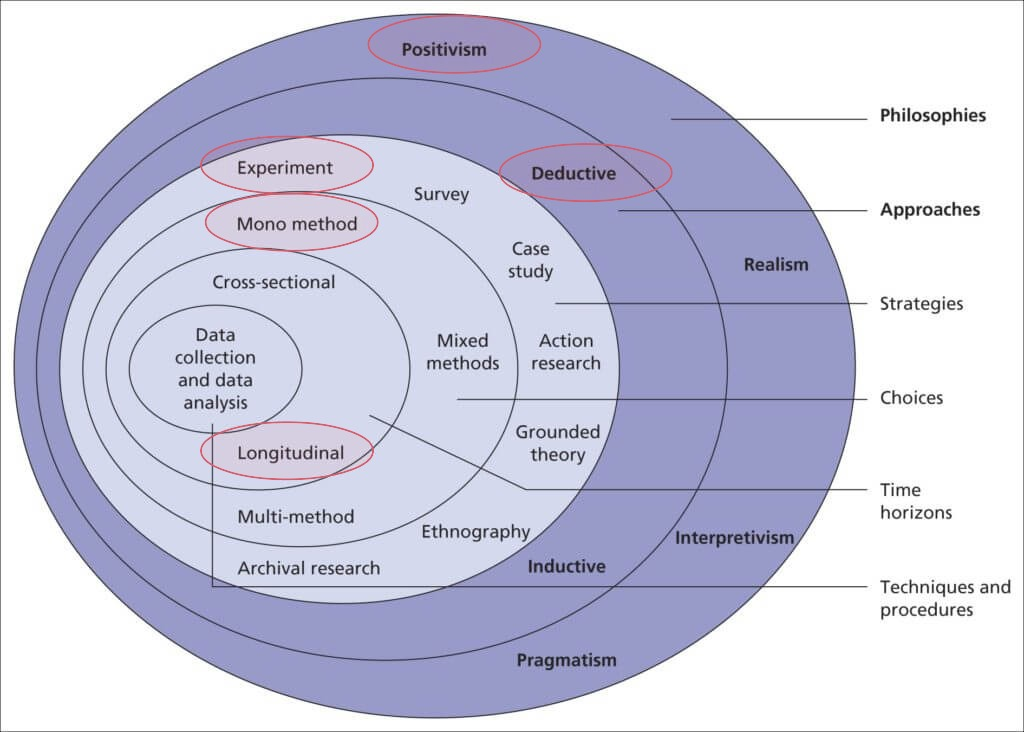
\includegraphics[width=\columnwidth]{includes/Research-Onion.jpg}
\caption{Research onion for the present study, adapted from Fig. 4.1 in Saunders, Lewis, and Thornhill \cite{saunders2007researchmethods}.}
\label{fig:research-design}
\end{figure}